\begin{figure}[!b]
\centering
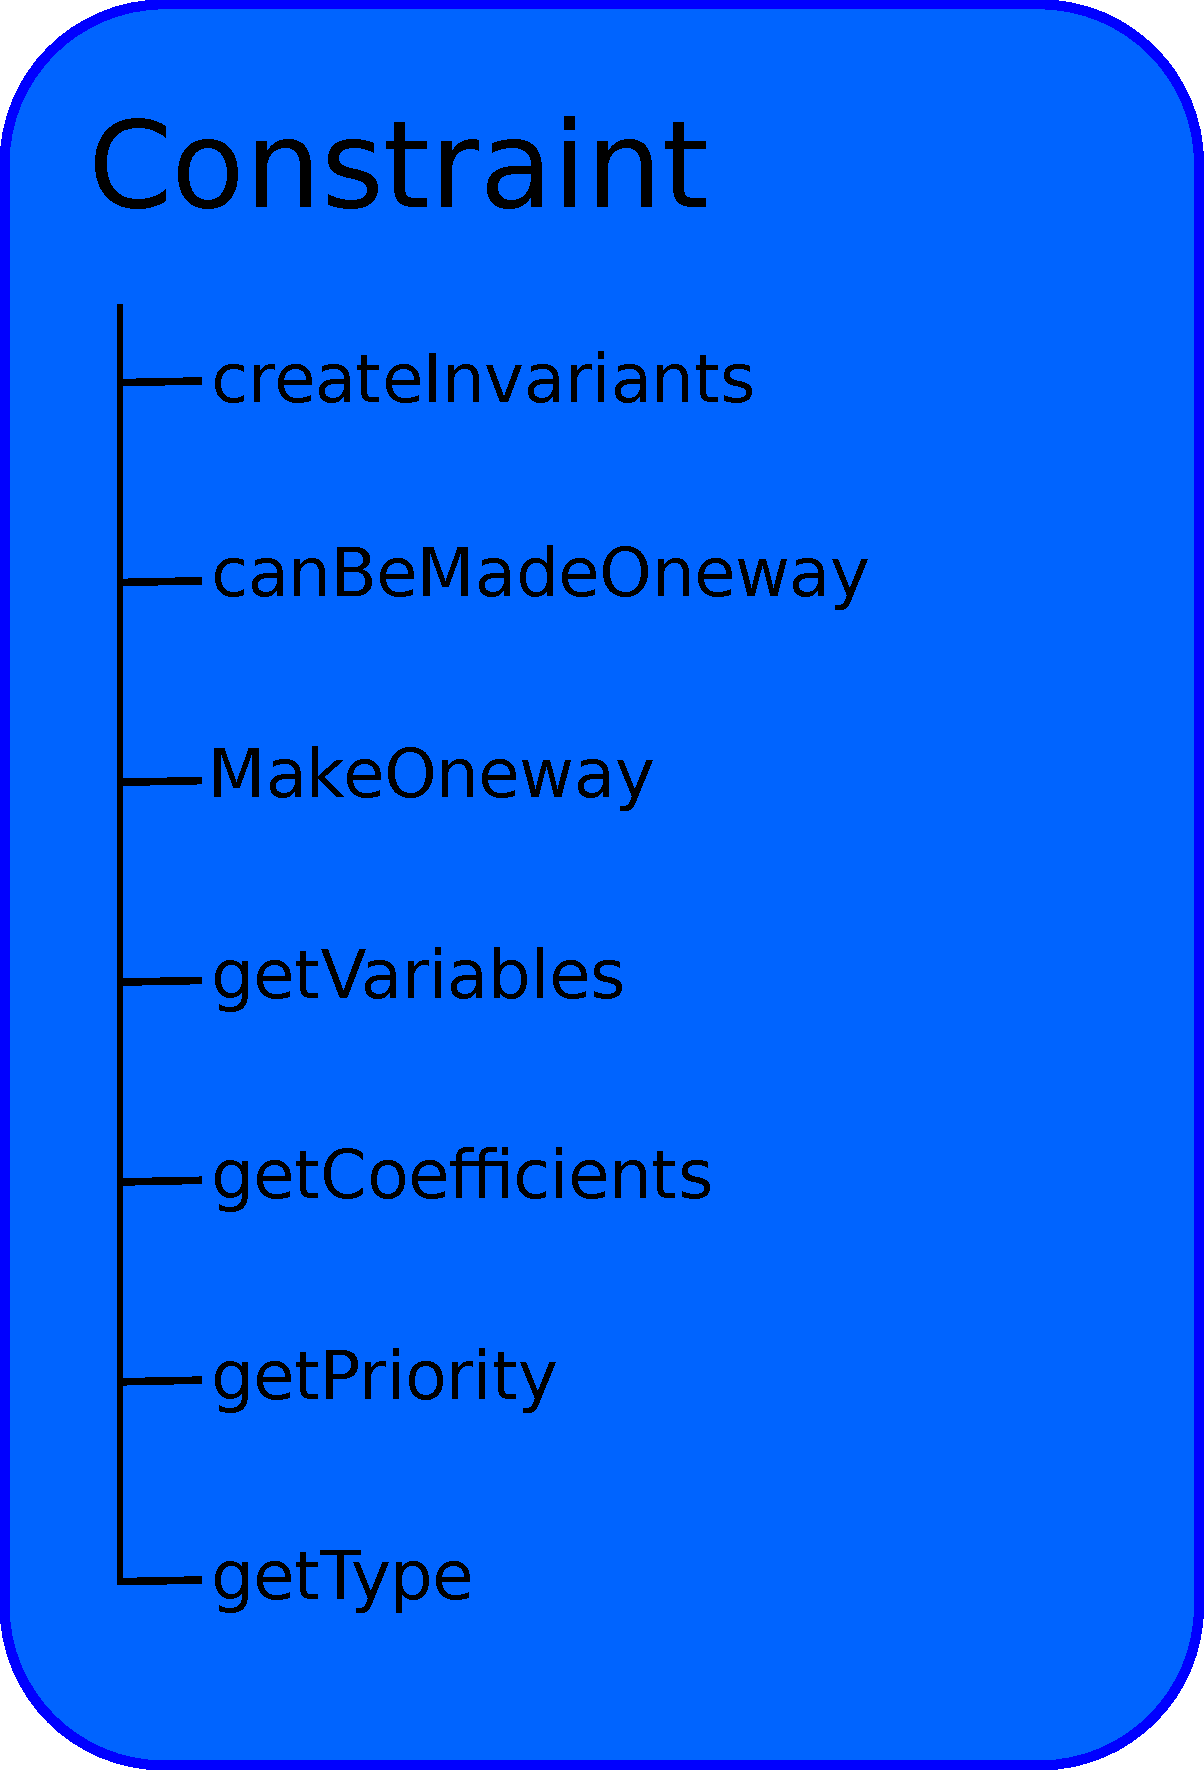
\includegraphics[width=\linewidth/2]{constraint.pdf} \caption{Important methods in Constraint 
class.}\label{fig_constraint}
% \end{center} 
\end{figure}
Constraints are all derived from the same class (\class{Constraint} figure \ref{fig_constraint}) which forces some 
methods to be implemented. All constraints need a priority according to how important the constraint is. The priority 
is given by an positive integer and do not need to be unique but it will help the local search differentiate between 
infeasible solutions. It is suggested to keep the size of the sequence of priorities lower than 5. \\
An example of a constraint is the \class{Linear} constraint, which is the same as the one used in integer and binary 
programming, equation $(5)$ is an example of a \class{Linear} constraint. 
\begin{equation}
 c_1: \; 2x_1 + 2x_2 \leq 2  \qquad x_1,x_2 \in \{0,1\}
\end{equation} \label{equat_linear} \noindent
A constraint is posted in the Gecode \class{Space} by \class{GecodeEngine} and later handled in the 
\class{LocalSearchEngine}. The constraints are treated differently in the environments and need different parameters and 
methods. The LS environment handles constraints through invariants hence an implementation of a constraint needs a 
method for creating the invariants needed in LS. The method \method{createInvariants} creates invariants that 
might be auxiliary variables helpful during local search and one invariant that represents 
whether the constraint is violated and the degree of violation. The degree of violation can be one if violated 
and zero otherwise, or it gives a measure of how violated the constraint is. For the linear constraint $c_1$ in 
equation $(5)$ the violation degree is how much the value of the left hand side must decrease to satisfy 
the 
constraint. A helpful auxiliary variable is the value of the left hand side such that it does not need to be recomputed 
when computing the violation. \\
The methods \method{canBeMadeOneway} and \method{makeOneway} are used if the constraint can be transformed 
to a oneway constraint hence functionally define one of the variables. Method \method{canBeMadeOneway} returns a 
boolean whether it can be used or not and \method{makeOneway} transforms the constriant into a oneway constraint, 
implemented as an invariant, that defines one of the variables. The only constraint that has been implemented is 
\class{Linear}. 
\subsubsection{Implementation of the Linear Constraint}
\class {Linear} is a linear constraint $c_j$ with a coefficient hashmap $A(c_j)$ and a vector of variables $X(c_j)$ 
that have some relation to a constant on the right hand side $b(c_j)$. The relation that can be used are
$\{\leq,=,\geq,>,<\}$ 
but only the first two $\{\leq,=\}$ needs to be managed. If any of the reamaining is used it is transformed into a 
less than or equal relation instead. The change can be done by multiplying with minus 1 on each side to change from a
``greater'' to a ``less'' relation. All coefficients and variables are integers hence all strictly less/greater 
relations can be transformed to a less/greater and equal relation by increasing or decreasing $b(c_j)$ by one. \\
The methods \method{canBeMadeOneway} and \method{makeOneway} are covered in section \ref{sec_ls} and only 
\class{Linear} constraints that have ``$=$'' relation can be made oneway constraints. \\ 
The method \method{createInvariants} creates two invariants; the first one represents the value of the left hand side 
in 
the constraint and the other represents the violation degree. The first invariant is a \class{Sum} invariant and is 
described in the next subsection. The second one depends on the relation of the constraint and is either a 
\class{LEQVioaltion} or 
\class{EQVioaltion} that are also describe in the next subsection. \\
If a variable is is defined by an invariant it belongs to the set $Y(c_j)$ instead of $X(c_j)$. Algorithm 
\ref{algo_lin} illustrates how the two invariants for \class{Linear} is created. \\
\IncMargin{1em}
\begin{algorithm}[H]

%\SetKwFunction{relation}{relation}\SetKwFunction{coeff}{coefficient}
  \algdata
\Input{\cons $c_j$}
\Output{two invariants}
\BlankLine
	set invars $= \emptyset$\;
%         set coef = getCoefficients() \;
        \class{Sum} y = Sum($A(c_j)$,$X(c_j)$,$Y(c_j)$)\;
         \int value = sumInvariant.setValue()\;
         invars.add(sumInvariant)\;
         \If{getPriority() $\neq$ 0 } {
                \eIf{relation \upshape is '$\leq$'}{
                    LEQviolation leq = LEQviolation(sumInvariant, $b(c_j)$)\;
                     \eIf{value $\leq$ $b(c_j)$}{
                         $V(leq) =0$\;
                      }{
                          $V(leq) =(value - rightHandSide)$\;
                     }
                    invars.add(leq)\;
                } {
                   EQviolation eq = EQviolation(sumInvariant, $b(c_j)$)\;
                   \eIf{value == $b(c_j)$} {
                       $V(eq) =0$\;
                   }{
                       $V(eq) =|value - rightHandSide|$)\;
                   }
                   invars.add(eq)\;
                }
         }

        \Return invars\;
    
   
   
\caption{Linear - createInvariants()} \label{algo_lin} 
 %\caption{Test if a constraint $c$ can define a variable $x$ } \label{algo_checkoneway}
\end{algorithm} \noindent
\DecMargin{1em} \\


